\chapter{Asking Dubai Supercar Owners How They Got RICH!}

This interview begins as spectacle and only gradually reveals its machinery. We are first shown finished symbols of wealth: a Rolls-Royce, a water-park empire, Jason Derulo, a \(\$600{,}000\) cash purchase, and finally a provocation about what banks quietly take away. Only after that does the lecture settle down and ask its real questions. What kind of business throws off this level of money? What sort of temperament survives bankruptcy, lawsuits, and public rejection? Why can an apparently dull business such as car washes become more structurally powerful than glamour itself? And, at the end, what does a small recurring drag do to compounding when we let it act over many periods? The lecture's rhythm is therefore deliberate: first the visible object, then the business mechanism, and only at the end the numerical spine.

\section{Dubai as Cold Open}

The lecture opens with a montage rather than an argument. A Rolls-Royce appears before we know the owner. The world's largest water park is named before we know the path that built it. Jason Derulo is identified before we are told that music is not the business we should be looking at. A final voice speaks of hundreds of millions, and another says that in Dubai many transactions happen in cash. The effect is not confusion but staging. We are meant to feel the finished scale of the outcome before we are shown the structure underneath it.

One of the first usable quantities is the price of the Rolls-Royce:
\begin{equation}
C_{\text{Rolls}}=\$600{,}000.
\end{equation}
At first this is merely a shock device. But the lecture immediately turns it into a question about transactional form. If a car at that scale is bought in cash, then the object itself is no longer the central fact. The central fact is the financial environment in which such a purchase can be made without ceremony.

\begin{figure}[h]
\centering
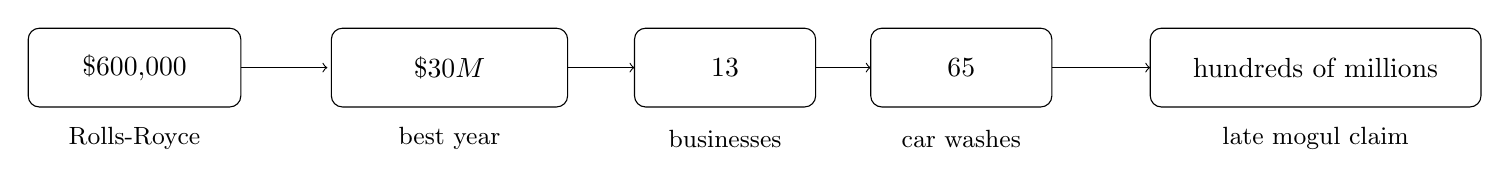
\begin{tikzpicture}[x=1cm,y=1cm]
\node[draw, rounded corners, minimum width=2.7cm, minimum height=1cm] (a) at (0,0) {\(\$600{,}000\)};
\node[draw, rounded corners, minimum width=3cm, minimum height=1cm] (b) at (4,0) {\(\$30\text{M}\)};
\node[draw, rounded corners, minimum width=2.3cm, minimum height=1cm] (c) at (7.5,0) {\(13\)};
\node[draw, rounded corners, minimum width=2.3cm, minimum height=1cm] (d) at (10.5,0) {\(65\)};
\node[draw, rounded corners, minimum width=4.2cm, minimum height=1cm] (e) at (15,0) {hundreds of millions};

\node at (0,-0.9) {\small Rolls-Royce};
\node at (4,-0.9) {\small best year};
\node at (7.5,-0.9) {\small businesses};
\node at (10.5,-0.9) {\small car washes};
\node at (15,-0.9) {\small late mogul claim};

\draw[->] (1.35,0) -- (2.45,0);
\draw[->] (5.5,0) -- (6.35,0);
\draw[->] (8.65,0) -- (9.35,0);
\draw[->] (11.65,0) -- (12.9,0);
\end{tikzpicture}
\caption{Transcript-based reconstruction of the lecture's cold open. The lecture first stacks price tags, annual incomes, and business counts, and only afterward begins to explain them.}
\end{figure}

Only after this does the host reset the scene in plain language. We are in Dubai. We will move through wealthy areas. We will stop owners and ask what they actually did to afford the machines in front of us. That reset matters. Without it the chapter would remain a collage. With it, the lecture becomes a search for mechanisms.

\section{The Water-Park Operator: Failure Counted Rather Than Hidden}

The first full case is the owner who says he runs the world's largest water park. The lecture could have used him as an exotic success story and moved on. Instead it does something much better. It almost immediately turns away from visible wealth and into accumulated damage. He says he has been bankrupt twice and sued twenty-four times:
\begin{equation}
N_{\text{bankruptcies}}=2,
\qquad
N_{\text{lawsuits}}=24.
\end{equation}
Then the pressure sharpens. He recalls seeing a message that left him
\begin{equation}
D_{\text{negative}}\approx -\$1.8\,\text{million}.
\end{equation}
For several years he was paying back debts connected to a former business partner. The lecture is already doing something important here. It is replacing vague inspiration with countable adversity. Bankruptcy is counted. Lawsuits are counted. Debt is counted. The point is not simply that he suffered. The point is that the business path can be read as a sequence of quantifiable blows that did not close the process.

Partner choice then enters the lecture as a first-order variable. He says he now prefers to play solo, even though he still does joint ventures. The reason is not a slogan about ownership. It is experience. He describes himself as aggressive, willing to fail, not frightened by temporary monetary loss. A partner who does not share that operating temperament is therefore not merely a stylistic mismatch. He is a structural risk.

\subsection{Question \& Answer}

\paragraph{Question.}
How does repeated failure become business capital rather than a stopping point?

\paragraph{Answer.}
The lecture's answer is severe rather than uplifting. Failure becomes usable only if the operator does not convert it into a final judgment on himself. Bankruptcy, lawsuits, and bad partners are not described as noble scars; they are described as expensive training. That is why the speaker can say that for him it is ``just money.'' He does not mean money is irrelevant. He means that he has learned to distinguish between temporary destruction of a balance sheet and permanent destruction of operating will.

The lecture then tightens this doctrine through rejection count:
\begin{equation}
N_{\text{rejections}}=617.
\end{equation}
Spread across a year, the implied pace is
\begin{equation}
r_{\text{rejections}}
\approx
\frac{617}{365}
\approx
1.69\ \text{per day}.
\end{equation}
The host rounds the idea upward into ``at least two no's'' each day. The arithmetic is not exact, but the lecture's intention is clear. Rejection is not theatrical. It is iterative.

The underlying update rule is therefore not psychological but procedural:
\begin{equation}
\text{attempt}\to \text{no}\to \text{learning}\to \text{next attempt}.
\end{equation}
Once we write it that way, the lecture's rhetoric becomes easier to understand. ``Every no'' is not celebrated for its own sake. It is valuable because it advances the search.

\section{Mindset, Debt Notes, and the Misreading of Wealth}

After the rejection count, the lecture adds a quieter but equally important layer. The same speaker recalls a note written to himself eight years earlier, when he had three legal cases on him and roughly a quarter million dollars in debt:
\begin{equation}
D_{\text{note}}\approx -\$250{,}000.
\end{equation}
What he reads out is not mathematics, but it behaves like a system of operating constraints. Train the mind harder than anyone else. Refuse another person's limitation. Accept pain. Visualize. Learn overload. Become obsessed. Never become satisfied. The lecture is careful to place this after the bankruptcy and rejection material. Otherwise mindset would sound like generic motivational padding. Here it reads instead as a set of instructions written under pressure, by someone who had already learned what weak structure costs.

\subsection{Question \& Answer}

\paragraph{Question.}
Is mindset really prior to skill, or only what survives after skill collapses?

\paragraph{Answer.}
The lecture's answer is that skill matters, but it is not the first thing to fail. Under legal pressure, debt, bad partnerships, and repeated rejection, skill by itself does not explain persistence. The note matters because it shows the speaker building a discipline for carrying pain over time. In that sense mindset is not magical and not decorative. It is the part of the system that remains operative when technique has not yet delivered a reward.

At this point the host steps back and performs one of the lecture's most important transitions. He says, in effect, that the first interview should correct a lazy stereotype. It is too easy to see Dubai or the UAE and assume inherited wealth. The water-park operator is presented as counterevidence: not born rich, not lifted by a family fortune, but built through counted adversity, repeated selling, and the refusal to stop. This recap is not repetition. It resets the reader's causal model before the next owner appears.

\section{Cash, Sacrifice, and the Price of the Future Self}

We now return to the Rolls-Royce, but the lecture wants a different lesson from it. The next entrepreneur says he owns a fashion brand called Icon, has been an entrepreneur for six years, and made
\begin{equation}
Y_{\text{fashion}}=\$30\,\text{million}
\end{equation}
in the present year. The host again asks the obvious Dubai question: was the Rolls-Royce bought in cash? The answer is yes, and the city is immediately used to frame the fact: many transactions happen in cash. So the same number,
\begin{equation}
C_{\text{Rolls}}=\$600{,}000,
\end{equation}
returns not simply as a price tag but as a local expression of how capital moves.

The deeper part of the interview, however, is not about payment form. It is about sacrifice. The speaker says that whatever we want can be had if we are willing to bleed for it. The lecture does not leave the word ``bleed'' in poetic suspension. It unpacks the cost into specific acts of subtraction: monk mode, isolation, refusal of distraction, willingness to trade present comfort for future identity. The governing claim is that ambition is not merely additive. It removes one life in order to make room for another.

\subsection{Question \& Answer}

\paragraph{Question.}
What price does the future self extract from the present self?

\paragraph{Answer.}
The lecture's answer is that the price is paid partly in money and partly in immediate recognizability. We do not only buy the desired future. We also surrender habits, social ease, romance, leisure, and the comfort of remaining the person we already know. That is why the speaker says dream life has a price. The price is not metaphorical. It is a transfer of present-life substance into future possibility.

The social corollary follows immediately. Haters are treated as normal structure, not unfortunate accident. In the speaker's account, many people attack what they themselves abandoned. If they see someone else still pursuing it, they respond to their own surrender. The lecture therefore widens again: social resistance is not evidence that the project is invalid. It is often one of the prices charged for staying in the game.

Before moving on, the lecture breaks for the host's community and mentor plug. This is not part of the mathematical core, but as pacing it matters. The temperature drops, the pitch resets, and the celebrity case can begin without being forced to carry the emotional residue of the previous one.

\section{Jason Derulo and the Car-Wash Machine}

Jason Derulo enters first as recognition and only then as mechanism. The host asks for the largest amount made in a single year, and the answer is
\begin{equation}
Y_{\text{Jason}}=\$30\,\text{million}.
\end{equation}
He also says he owns about thirteen businesses:
\begin{equation}
N_{\text{businesses}}\approx 13.
\end{equation}
The real reveal comes when the host asks which business made the most money. It is not music. It is car washes. The count is substantial:
\begin{equation}
N_{\text{car washes}}\approx 65.
\end{equation}

Now the lecture becomes more explicit about business structure. Car washes, he says, are powerful because they combine two clocks. On one clock they are daily-use operating assets: people wash their cars repeatedly, and the car itself functions as a visible extension of identity and success. On another clock they are land: the site itself appreciates over time. A third layer is added through customer experience. Better service, more attention to detail, and the treatment of every visit as if it were the last chance to keep that customer all increase the durability of the machine.

We should not turn this into a pretend valuation model with cap rates and operating statements the lecture never gives. But we can write its structure honestly:
\begin{equation}
V_{\text{car wash}}
\approx
V_{\text{land}}
+
V_{\text{recurring demand}}
+
V_{\text{service reputation}}.
\end{equation}
This is not a theorem. It is a faithful compression of the explanation the speaker gives. The point is that the apparently boring business wins because it binds together land, routine use, and disciplined customer retention.

\begin{figure}[h]
\centering
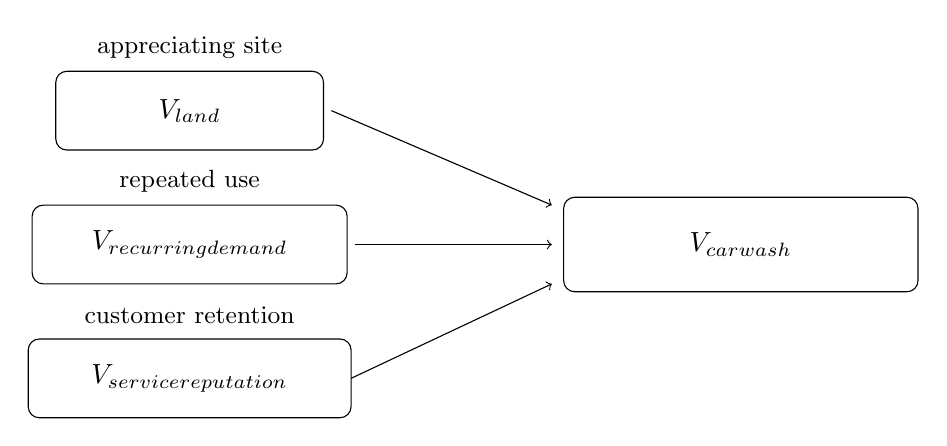
\begin{tikzpicture}[x=1cm,y=1cm]
\node[draw, rounded corners, minimum width=3.4cm, minimum height=1cm] (land) at (0,0) {\(V_{\text{land}}\)};
\node[draw, rounded corners, minimum width=4cm, minimum height=1cm] (demand) at (0,-1.7) {\(V_{\text{recurring demand}}\)};
\node[draw, rounded corners, minimum width=4.1cm, minimum height=1cm] (service) at (0,-3.4) {\(V_{\text{service reputation}}\)};
\node[draw, rounded corners, minimum width=4.5cm, minimum height=1.2cm] (total) at (7,-1.7) {\(V_{\text{car wash}}\)};

\draw[->] (1.8,0) -- (4.6,-1.2);
\draw[->] (2.1,-1.7) -- (4.6,-1.7);
\draw[->] (2.05,-3.4) -- (4.6,-2.2);

\node at (0,0.8) {\small appreciating site};
\node at (0,-0.9) {\small repeated use};
\node at (0,-2.6) {\small customer retention};
\end{tikzpicture}
\caption{Transcript-based reconstruction of the car-wash explanation. The business is profitable not by glamour but by the interaction of land, recurring use, and customer experience.}
\end{figure}

\subsection{Question \& Answer}

\paragraph{Question.}
Why can a boring, land-backed business outperform glamour?

\paragraph{Answer.}
Because glamour is not itself a compounding structure. The lecture's surprise is that the famous person is not making the clearest money through the glamorous part of his life. The stronger machine is the one tied to repeated necessity, visible habit, and appreciating land. If a business earns on both the operating side and the asset side, it can outlast the symbolic aura that first brought attention to the operator.

The speaker calls the business recession-proof and pandemic-proof, at least in his experience. We should keep that attributed rather than universal. But it fits the lecture's broader movement: the hidden engine of wealth is often steadier, duller, and more structural than the visible surface.

\section{Negotiation, Delay, and the Refusal of Desperation}

Once the lecture has made the car-wash model legible, it shifts from business structure to operating conduct. The host asks for negotiation advice, and Jason Derulo gives a sequence rather than a slogan. First, let the other side make the initial offer. Only after that should we answer, and when we answer we should come back higher. In compact form,
\begin{equation}
a_{\text{other first}}
\to
a_{\text{counter}} > a_{\text{other first}}.
\end{equation}
The point is not cleverness for its own sake. It is to avoid injuring ourselves by naming a lower number than the market might have given us.

He then adds the second move. If the negotiation stalls, do not instantly chase the deal. Let time pass. Return later. The lecture's procedure can therefore be summarized as
\begin{equation}
\text{offer}\to \text{counteroffer}\to \Delta t_{\text{pause}}\to \text{return without desperation}.
\end{equation}
This is psychologically simple and commercially important. Neediness narrows the field of possible terms. The lecture therefore implies the heuristic
\begin{equation}
P_{\text{negotiation strength}}\uparrow
\qquad\text{as}\qquad
\text{neediness}\downarrow.
\end{equation}

\subsection{Question \& Answer}

\paragraph{Question.}
How do we negotiate from strength before we feel powerful?

\paragraph{Answer.}
The lecture's answer is procedural rather than emotional. We do not wait for an internal sensation of power. We arrange the interaction so that our weakness is not cheaply legible. Let the other side reveal an anchor. Counter rather than confess. Insert time rather than panic. Refuse the tempo of begging. Strength, on this view, is not first a mood. It is an order of operations.

The section then widens one last time. Jason's advice to his younger self is that what we are not changing, we are choosing. This turns a negotiation lesson into a general law of agency. The issue is not only how to secure a better deal. It is whether we are acting at all on conditions we claim to dislike.

\section{Compounding Drag and the Preservation of the Base}

The lecture's final major speaker is where it becomes most explicitly mathematical. The host asks what lesson about money banks do not want people to know. The first answer is rhetorical: a small annual skim may silently absorb most of what a life of compounding would otherwise have produced. That rhetorical version is too loose to formalize directly. So the lecture itself tightens. It gives us a simpler and cleaner example.

We start with
\begin{equation}
W_0=\$1,
\qquad
n=20,
\qquad
\tau=25\%.
\end{equation}
The undragged case is straightforward:
\begin{equation}
W_n=W_0\,2^n.
\end{equation}
At \(n=20\), this yields
\begin{equation}
W_{20}=2^{20}=\$1{,}048{,}576.
\end{equation}
This is the exact completion of the speaker's rounded \(\$1{,}048{,}000\).

Now we impose the drag. Gross doubling means that in each period the profit equals the current base \(W_k\). If a quarter of that profit is taken away, the retained profit is \((1-\tau)W_k\). Therefore the wealth update rule becomes
\begin{align}
W_{k+1}
&=
W_k+(1-\tau)W_k \\
&=
(2-\tau)W_k.
\end{align}
With \(\tau=0.25\), we obtain
\begin{equation}
W_{k+1}=1.75\,W_k,
\end{equation}
and so
\begin{equation}
W_{20}^{(\tau=0.25)}=1.75^{20}\approx \$72{,}571.
\end{equation}
The speaker gives a rough endpoint of \(\$50{,}000\) to \(\$70{,}000\). The exact standard reconstruction lands slightly above that interval, but it preserves the lecture's real point: the drag is not destructive because it subtracts a lot once. It is destructive because it slows the growth of the base at every step.

The ratio of dragged to undragged wealth is
\begin{equation}
\frac{W_{20}^{(\tau=0.25)}}{W_{20}}
\approx
\frac{72{,}571}{1{,}048{,}576}
\approx
0.0692.
\end{equation}
So only about \(6.9\%\) of the original endpoint remains, and the loss fraction is
\begin{equation}
1-0.0692\approx 0.9308.
\end{equation}
In other words, the final amount is roughly \(93\%\) lower. The lecture says \(96\%\), and that figure should be heard as rhetorical emphasis rather than as exact arithmetic.

\begin{figure}[h]
\centering
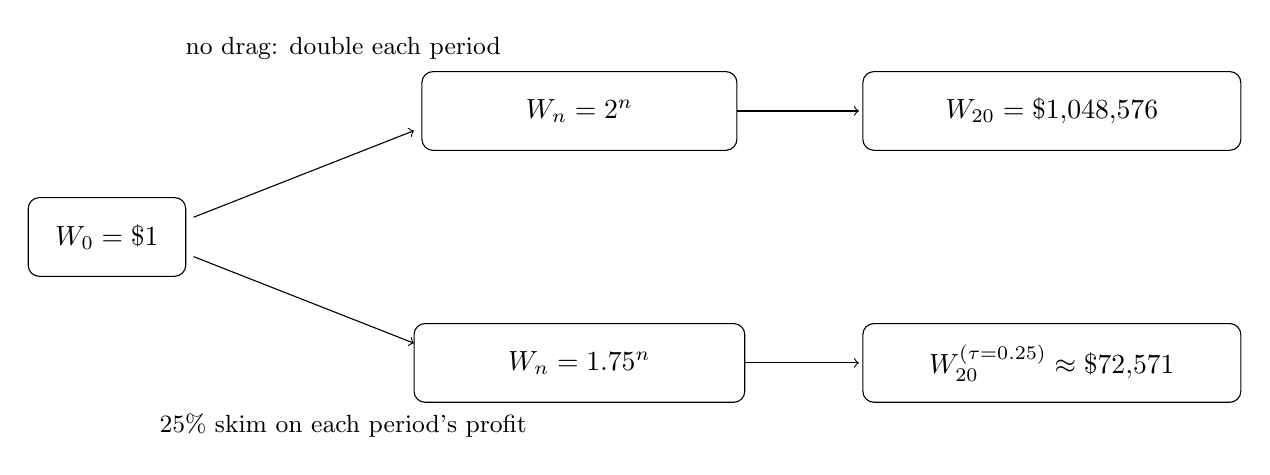
\begin{tikzpicture}[x=1cm,y=1cm]
\node[draw, rounded corners, minimum width=2cm, minimum height=1cm] (start) at (0,0) {\(W_0=\$1\)};
\node[draw, rounded corners, minimum width=4cm, minimum height=1cm] (top) at (6,1.6) {\(W_n=2^n\)};
\node[draw, rounded corners, minimum width=4.2cm, minimum height=1cm] (bottom) at (6,-1.6) {\(W_n=1.75^n\)};
\node[draw, rounded corners, minimum width=4.8cm, minimum height=1cm] (topend) at (12,1.6) {\(W_{20}=\$1{,}048{,}576\)};
\node[draw, rounded corners, minimum width=4.8cm, minimum height=1cm] (botend) at (12,-1.6) {\(W_{20}^{(\tau=0.25)}\approx \$72{,}571\)};

\draw[->] (1.1,0.25) -- (3.9,1.35);
\draw[->] (1.1,-0.25) -- (3.9,-1.35);
\draw[->] (8,1.6) -- (9.55,1.6);
\draw[->] (8.1,-1.6) -- (9.55,-1.6);

\node at (3,2.4) {\small no drag: double each period};
\node at (3,-2.4) {\small \(25\%\) skim on each period's profit};
\end{tikzpicture}
\caption{Transcript-based reconstruction of the compounding comparison. The drag does not merely subtract from one round; it changes the multiplier acting on all future rounds.}
\end{figure}

\subsection{Question \& Answer}

\paragraph{Question.}
Why can a small recurring drag destroy almost the entire endpoint of compounding?

\paragraph{Answer.}
Because compounding does not act on a fixed amount. It acts on a base that is itself growing. Once we diminish that base at every stage, every future multiplication occurs on a weakened platform. The real loss is therefore not the first subtraction by itself. The real loss is the destruction of the later rounds that would have been built on what was removed.

The lecture does not stop with the arithmetic. It immediately turns the same logic into negotiation. The final speaker says that business negotiations are won by people who do not need the deal, then complicates the line by admitting that real situations often involve genuine need. His own example stretches across roughly
\begin{equation}
\Delta t_{\text{deal}}\approx 8\text{ to }9\ \text{months}.
\end{equation}
Late in that process, investors insist on a contractual clause he does not want. Lawyers and bankers are present; the deal is tense and large. He asks for a break. Outside the room, he tells his own advisers that the deal may be off. They think he is making a disastrous mistake.

The decisive move comes only after he returns. He does not argue about the clause in isolation. He reframes the problem from the other side's future perspective. If they will become his shareholders after the deal, then what kind of CEO should they want? One who caves under pressure, or one who refuses terms that are bad for the shareholders he represents? In compact form, the lecture's logic can be rendered as
\begin{equation}
\text{if }U_{\text{shareholders}}(\text{accept clause})
<
U_{\text{shareholders}}(\text{walk away}),
\text{ reject the deal.}
\end{equation}
The notation is ours, not his, but the logic is his exactly. The question is not whether he can dominate the room theatrically. The question is whether he will preserve the future base of shareholder value rather than trade it away for a local concession.

Then he falls quiet. That silence is part of the lecture's rhythm and should be kept in mind. He has done the work of reframing. He now lets the other side inhabit the future he has described. The same instinct governs both halves of the section. In the mathematics, preserve the base. In negotiation, preserve the enterprise that the deal is supposed to protect.

\section{Summary}

The lecture begins with supercars and ends with compounding, but its internal motion is coherent all the way through. First we are shown wealth as a visible object. Then the lecture strips away the object and gives us a sequence of mechanisms: partner risk, counted failure, rejection as iteration, mindset under debt, sacrifice of present identity, dull but structurally powerful land-backed businesses, negotiation without desperation, and finally a clean numerical warning about what recurring drag does to the endpoint of growth. If there is a single lesson running underneath all of it, it is that wealth here is never treated as a mysterious aura. It is treated as a structure that can be built, damaged, defended, and, if we are careless, quietly bled away.